% !TeX TS-program = xelatex
\documentclass[aspectratio=169, 12pt, xcolor=table]{beamer}
\usefonttheme{professionalfonts}
\usefonttheme{serif}
\usepackage[T1]{fontenc}
\usepackage{fontspec-xetex}

\usepackage{tikz}

\usepackage{booktabs}
\usepackage{listings}
\usepackage{subcaption}

\usetikzlibrary{shapes.geometric, arrows}

\setmainfont{Lato}

%\PassOptionsToPackage[more=table]{xcolor}

% Local configuration
\renewcommand{\figurename}{}
\DeclareCaptionFormat{custom}
{%
	\tiny #3
}
\captionsetup{format=custom}

% Title stuff
\title{Programming}
\subtitle{Flow Control}
\date{Week 02}
\author{Vassilis Markos, Mediterranean College}

\usetheme{streamline}

% Local Commands
\newcommand{\ohref}[1]{\href{#1}{\texttt{#1}}}

% Code listings

\definecolor{codegreen}{rgb}{0,0.6,0}
\definecolor{codegray}{rgb}{0.5,0.5,0.5}
\definecolor{codepurple}{rgb}{0.58,0,0.82}
\definecolor{backcolour}{rgb}{0.95,0.95,0.92}

\lstdefinestyle{mystyle}{
	backgroundcolor=\color{backcolour},   
	commentstyle=\color{codegreen},
	keywordstyle=\color{magenta},
	numberstyle=\tiny\color{codegray},
	stringstyle=\color{codepurple},
	basicstyle=\ttfamily\footnotesize,
	breakatwhitespace=false,         
	breaklines=true,                 
	captionpos=b,                    
	keepspaces=true,                 
	numbers=left,                    
	numbersep=5pt,                  
	showspaces=false,                
	showstringspaces=false,
	showtabs=false,                  
	tabsize=2
}

\lstset{style=mystyle}

% Tikz style

\tikzstyle{startstop} = [ellipse, rounded corners, minimum width=2cm, minimum height=0.8cm, text centered, draw=black, fill=none]
\tikzstyle{io} = [trapezium, trapezium left angle=70, trapezium right angle=110, minimum width=2cm, minimum height=0.8cm, text centered, draw=black, fill=none]
\tikzstyle{process} = [rectangle, minimum width=2cm, minimum height=0.8cm, text centered, draw=black, fill=none]
\tikzstyle{decision} = [diamond, minimum width=2cm, minimum height=0.8cm, text centered, draw=black, fill=none]
\tikzstyle{arrow} = [thick,->,>=stealth]

% makeatletter stuff

\makeatletter
\newcommand{\arabicthree}[1]{\expandafter\@arabicthree\csname c@#1\endcsname}
\newcommand{\@arabicthree}[1]{\ifnum #1<100 0\fi\ifnum #1<10 0\fi\number#1}
\makeatother

\newcounter{exno}
\setcounter{exno}{0}

\newcommand{\exno}{\stepcounter{exno}In--class Exercise \#\arabicthree{exno}}

\begin{document}

	\begin{frame}
		\titlepage
	\end{frame}

	\begin{frame}{Contents}
		\tableofcontents
	\end{frame}

%	\section{A Brief Intro}\label{sec:a-brief-intro}
%	
%	\sectionframe
%	
%	\begin{headsup}{Desperate Times, Desperate Measures}
%		\begin{minipage}[t]{0.40\textwidth}
%			\vspace{0pt}
%			Since we are transitioning on a new platform, things are still a bit quirky. So, to make sure we keep track of who is here and who is not, please \textbf{scan the QR code shown next} or \textbf{click the link below it} and fill in this form with your information (confidential).
%		\end{minipage}\hfill
%		\begin{minipage}[t]{0.58\textwidth}
%			\vspace{0pt}
%			\raggedleft
%			
\includegraphics[scale=0.35]{../../assets/attendance_form.png}
%			\centering
%			\ohref{https://forms.gle/4yiYhonrjuVs4sCv6}
%		\end{minipage}
%	\end{headsup}
%
%	\begin{headsup}{Desperate Times, Desperate Measures}
%		\begin{minipage}[t]{0.50\textwidth}
%			\vspace{0pt}
%			For similar reasons, we will also be using a public shared drive folder to keep our materials as long as our platform is a bit unstable. To visit the platform and download this lecture's materials please use the QR shown right or the link below.
%		\end{minipage}\hfill
%		\begin{minipage}[t]{0.48\textwidth}
%			\vspace{0pt}
%			\raggedleft
%			
\includegraphics[scale=0.25]{../../assets/shared_folder.png}
%			\centering
%		\end{minipage}
%		\vfill
%		\begin{scriptsize}
%			\ohref{https://drive.google.com/drive/folders/1cUY\_XNJLyGNHRRgfJbxXemf8AFgiMnaF?usp=sharing}
%		\end{scriptsize}
%	\end{headsup}

	\section{Branching}\label{sec:branching}
	
	\sectionframe
	
	\begin{frame}{Python Environment}
		\begin{figure}
			\centering
			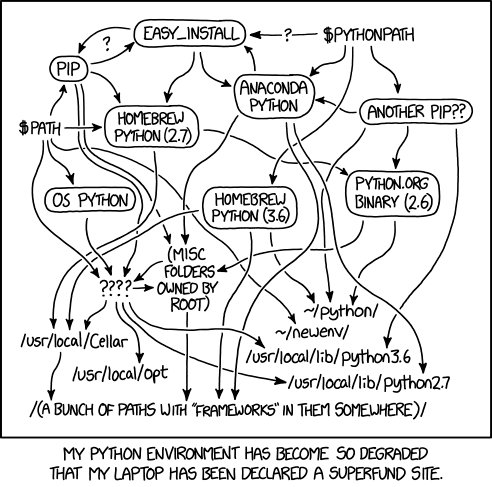
\includegraphics[height=0.65\textheight]{./assets/python_environment.png}
			\caption{Tidy up your Python environment regularly. Source: \ohref{https://xkcd.com/1987/}.}
		\end{figure}
	\end{frame}
	
	\begin{frame}{Even Or Odd?}
		How does the following program work?
		\lstinputlisting[language=Python]{../source/flow_control_001.py}
	\end{frame}

	\begin{frame}{Sequential Coding}
		\begin{minipage}{0.6\textwidth}
			\vspace{0pt}
			\begin{itemize}
				\item Consider the following program:
				\lstinputlisting[language={Python}]{../source/sequential.py}
				\item In the above, the code is executed \textbf{sequentially}, i.e., one line after the other.
			\end{itemize}
		\end{minipage}\hfill
		\begin{minipage}{0.38\textwidth}
			\vspace{0pt}
			\begin{center}
				\scalebox{0.65}{%
				\begin{tikzpicture}
					\node[startstop] (start) at (0,0) {start};
					\node[io] (input) at (0,-2) {\texttt{n = int(input(...))}};
					\node[process] (process) at (0,-4) {\texttt{m = -n}};
					\node[io] (output) at (0,-6) {\texttt{print(m)}};
					\node[startstop] (stop) at (0,-8) {stop};
					\draw[arrow] (start) -- (input);
					\draw[arrow] (input) -- (process);
					\draw[arrow] (process) -- (output);
					\draw[arrow] (output) -- (stop);
				\end{tikzpicture}}
			\end{center}
		\end{minipage}
	\end{frame}

	\begin{frame}{Branching}
		\begin{minipage}{0.6\textwidth}
			\vspace{0pt}
			\begin{itemize}
				\item Consider the following program:
				\lstinputlisting[language={Python}]{../source/flow_control_001.py}
				\item Here we need to change path upon a condition. This is called \textbf{branching}.
			\end{itemize}
		\end{minipage}\hfill
		\begin{minipage}{0.38\textwidth}
			\vspace{0pt}
			\begin{center}
				\scalebox{0.65}{%
					\begin{tikzpicture}
					\node[startstop] (start) at (0,0) {start};
					\node[io] (input) at (0,-2) {\texttt{n = int(input(...))}};
					\node[decision, aspect=2] (condition) at (0,-4) {\texttt{n \% 2 == 0}};
					\node[io] (even) at (-2,-6) {\texttt{"even"}};
					\node[io] (odd) at (2,-6) {\texttt{"odd"}};
					\node[startstop] (stop) at (0,-8) {stop};
					\draw[arrow] (start) -- (input);
					\draw[arrow] (input) -- (condition);
					\draw[arrow] (condition) -- (even) node[pos=0.5, fill=white] {True};
					\draw[arrow] (condition) -- (odd) node[pos=0.5, fill=white] {False};
					\draw[arrow] (even) -- (stop);
					\draw[arrow] (odd) -- (stop);
					\end{tikzpicture}}
			\end{center}
		\end{minipage}
	\end{frame}

	\begin{frame}{Another Example Of Branching}
		What will the following program print?
		\lstinputlisting[language={Python}]{../source/flow_control_002.py}
	\end{frame}

	\begin{headsup}{Python And Indentation}
		\textbf{In Python, whitespace matters!}
		\begin{itemize}
			\item Whenever we enter a new code block we must indent our code accordingly.
			\item Usually, we use the \texttt{Tab} character to make sure all our code is properly indented.
			\item In case code is not properly indented, Python will raise an error (recall last lecture's lab).
			\item Most modern text editors take care of indentation and enter a \texttt{Tab} automatically when entering a code block.
		\end{itemize}
	\end{headsup}

	\begin{frame}{Multiple Branches}
		What will the following print?
		\lstinputlisting[language={Python}]{../source/flow_control_003.py}
	\end{frame}

	\begin{frame}{Complex Branching In Python}
		Python offers a general purpose \texttt{if-elif-\ldots-else} construct. The way this is interpreted is as follows:
		\begin{enumerate}
			\item First, the \texttt{if} condition is checked. If it is satisfied, the interpreter exits the block.
			\item\label{item:step} If the \texttt{if} condition fails, the interpreter proceeds with the first \texttt{elif} condition. If successful, it exits the block.
			\item Step~\ref{item:step} is repeated until all \texttt{elif} statements have been checked and failed or one has been successful.
			\item If none \texttt{if} / \texttt{elif} statement has been successful, the \texttt{else} case is executed (if there is one).
		\end{enumerate}
	\end{frame}

	\begin{frame}{Condition Simplification}
		Will this work the same as the previous one?
		\lstinputlisting[language={Python}]{../source/flow_control_003a.py}\pause
		Why is that?
	\end{frame}

	\begin{frame}{Condition Simplification}
		\begin{itemize}
			\item Each \texttt{elif} / \texttt{else} statement is executed on condition that all previous ones have failed.
			\item This means we do not need to specify in subsequent \texttt{elif} statements that the above ones have failed, as the interpreter would not have reached that point in our code otherwise.
			\item Use this as a \textbf{good practice} to make your code easier to read / share / maintain!
		\end{itemize}
	\end{frame}

	\begin{frame}{Condition Simplification}
		Simplify the conditions of the following program as much as possible:
		\lstinputlisting[language={Python}]{../source/flow_control_004.py}
	\end{frame}

	\begin{frame}{Condition Simplification}
		Rewrite the following using only \texttt{<} as a comparison operator, i.e., no \texttt{==}, \texttt{<=}, \texttt{>=} etc:
		\lstinputlisting[language={Python}]{../source/flow_control_005.py}
	\end{frame}
	
	\begin{frame}{\texttt{Bye!}}
		For which values of \texttt{n} will the following print \texttt{Bye!}?
		\lstinputlisting[language={Python}]{../source/flow_control_006.py}
	\end{frame}

	\begin{frame}{\texttt{Fry!}}
		For which values of \texttt{n} will the following print \texttt{Fry!}?
		\lstinputlisting[language={Python}]{../source/flow_control_007.py}
	\end{frame}
	
	\begin{frame}{What Is A Leap Year?}
		A leap year is a year which:\pause
		\begin{itemize}
			\item Is divisible by 4, but\ldots\pause
			\item is not divisible by 100, except for\ldots\pause
			\item when it is also divisible by 400.\pause
		\end{itemize}
		So, 2020 was a leap year, 2024 too, 2100 will not be, but 2000 was.
		
		Write a Python program that asks the user for a year and prints whether it is a leap year or not.
	\end{frame}

	\begin{frame}{Leap Years}
		One possible solution is shown below:
		\lstinputlisting[language={Python}]{../source/flow_control_008.py}\pause
		Can you use a shorter condition?
	\end{frame}

	\begin{frame}{Leap Years}
		Another way to deal with this:
		\lstinputlisting[language={Python}]{../source/flow_control_009.py}
	\end{frame}

	\begin{headsup}{Tips And Tricks}
		\begin{itemize}
			\item When dealing with really complex conditions, as in the previous case, we can split them using a more length \texttt{if-elif-\ldots-else} statement.
			\item This is not a general piece of advice: use with caution as it may result to really length code.
			\item However, in some cases, this makes code easier to read / share / maintain.
			\item Yet, in other cases we might end up with much redundant code, so\ldots
		\end{itemize}
	\end{headsup}

	\begin{frame}{Grades}
		Grades (0--100) correspond to A--F grades according to the following rule:
		\begin{itemize}
			\item A: 90-100
			\item B: 80-89
			\item C: 70-79
			\item D: 60-69
			\item F: 0-59
		\end{itemize}
		Write a Python program that asks the user for their grade in 0--100 and returns the corresponding A--F grade.
	\end{frame}

	\begin{frame}{A Possible Solution}
		\lstinputlisting[language={Python}]{../source/flow_control_010.py}
	\end{frame}
	
	\begin{frame}{Taxes}
		In Pythonland, taxes are collected according to the following scheme:
		\begin{itemize}
			\item First $10,000\$$ are free of tax.
			\item The next $5,000\$$ are taxed with a $5\%$ fee.
			\item The next $15,000\$$ are taxed with a $20\%$ fee.
			\item Any remaining income is taxed with a $40\%$ fee.
		\end{itemize}
		Write a Python program that asks the user for their income and computes their total tax fee.
	\end{frame}

	\begin{frame}{A Possible Solution}
		\lstinputlisting[language={Python}]{../source/flow_control_011.py}
	\end{frame}

	\begin{frame}{Some Remarks}
		\begin{itemize}
			\item Observe how in each case, we do not check whether the previous ones have failed, as we know that this is true (as discussed before).
			\item Also, since each portion of one's income is taxed differently, we have in each case to make use of the adequate formula for amounts that fall into one of the lower categories:
			\begin{itemize}
				\item For instance, for an income of $14,000\$$, the first $10,000\$$ are free of tax, while the remaining $4,000\$$ are taxed with a $5\%$ fee.
				\item For instance, for an income of $24,000\$$, the first $10,000\$$ are free of tax, while the remaining $14,000\$$ are taxed as follows: the first $5,000\$$ with a $5\%$ fee and the remaining $9,000\$$ with a $20\%$ fee.
			\end{itemize}
		\end{itemize}
	\end{frame}

	\section{Loops (First Try)}\label{sec:loops--first-try}
	
	\sectionframe
	
	\begin{frame}{Checking User Input}
		Assume that you want to write a program that decides whether a student has passed their exams. This could look like something we have seen above:
		\lstinputlisting[language={Python}]{../source/flow_control_002.py}
	\end{frame}

	\begin{frame}{Checking User Input}
		This is really nice, but what if a user enters a number outside the range $[0,100]$?\pause
		\lstinputlisting[language={Python}]{../source/flow_control_012.py}
	\end{frame}

	\begin{frame}{Users: The Source of All Bad}
		Run \texttt{../source/flow\_control\_012.py} and provide the following inputs:
		\begin{itemize}
			\item First, enter 115.
			\item Then, once prompted to enter your grade again, enter -56.
			\item What happened now?
			\item How can we prevent this, as well?
		\end{itemize}
	\end{frame}
	
	\begin{frame}{How About This?}
		\lstinputlisting[language={Python}]{../source/flow_control_013.py}
	\end{frame}

	\begin{frame}{Well\ldots}
		\begin{itemize}
			\item While the chances that a user makes twice the same mistake are quite low, they are not null.
			\item This means that we should also take care of the case where a user enters wrong input three times.
			\item Even worse: four or even five times! Let alone six!
			\item How can we handle this?
		\end{itemize}
	\end{frame}

	\begin{frame}{Repeated Branching}
		\begin{minipage}{0.6\textwidth}
			\vspace{0pt}
			\begin{itemize}
				\item What we actually need is something like what is shown in the next flow chart, where we keep visiting our condition until it becomes \texttt{False}.
				\item In programming, this is called a \textbf{loop}.
				\item Loops are really necessary in almost any realistically useful program, so we have to master them!
			\end{itemize}
		\end{minipage}\hfill
		\begin{minipage}{0.38\textwidth}
			\vspace{0pt}
			\begin{center}
				\scalebox{0.55}{%
					\begin{tikzpicture}
					\draw[dashed, rounded corners, thick, streamlineorange, fill=streamlineorange!10] (-3.5,-7.8) rectangle (2.6,-2.5);
					\node[startstop] (start) at (0,0) {start};
					\node[process] (a) at (0,-1.5) {\texttt{'Stuff'}};
					\node[decision, aspect=2.5, fill=white] (condition) at (0,-4) {\texttt{loop condition}};
					\node[process, fill=white] (inside) at (0,-7) {\texttt{"inside loop"}};
					\node[process] (outside) at (0,-8.5) {\texttt{"outside loop"}};
					\node[startstop] (stop) at (0,-10) {stop};
					\draw[arrow] (start) -- (a);
					\draw[arrow] (a) -- (condition);
					\draw[arrow] (condition.270) -- (inside.90) node[pos=0.5, fill=streamlineorange!10] {True};
					\draw[arrow] (condition.0) -- ++(1,0) -- ++(0,-4.5) node[pos=0.5, fill=white] {False} -- (outside.0);
					\draw[arrow] (outside) -- (stop);
					\draw[arrow] (inside.180) -- ++(-1.5,0) -- ++(0,3) -- (condition.180);
					\end{tikzpicture}}
			\end{center}
		\end{minipage}
	\end{frame}

	\begin{frame}{A Simple Python Loop}
		So, the above program can be efficiently written as follows:
		\lstinputlisting[language={Python}]{../source/flow_control_014.py}
	\end{frame}

	\begin{frame}[fragile]{Python \texttt{while} Loop Syntax}
		In Python, a \texttt{while} loop adheres to the following syntax:
		\begin{verbatim}
while <some logical condition>:
    <Stuff to be repeated while the condition holds>
\end{verbatim}
	\begin{itemize}
		\item Each \texttt{while} loop starts with the \textbf{\texttt{while}} keyword followed by a logical condition, i.e., a Python expression evaluating to \texttt{True} / \texttt{False}.
		\item Then, we have to use a colon (\texttt{:}) to denote that the loop declaration line has ended.
		\item Below we write any code we want to repeat \textbf{properly indented.}
	\end{itemize}
	\end{frame}
	
	\begin{headsup}{Important Notes}
		\begin{itemize}
			\item It is important to somehow \textbf{change} variables appearing in \textbf{a loop's logical condition!} Why?\pause
			\item Otherwise, the condition will never change from \texttt{True} to \texttt{False}, so we will end up with an \textbf{infinite loop.}\pause
			\item Similarly, it is important to make sure the loop condition evaluates to \texttt{True} at some time, otherwise we will never enter the loop.\pause
			\item As a consequence of the above, \texttt{while} loops might never be executed (bug or feature, depending on our purpose) on some occasions.
		\end{itemize}
	\end{headsup}

	\begin{frame}{Booleanity In Python}
		What will the following print?
		\lstinputlisting[language={Python}]{../source/flow_control_015.py}\pause
		The above results to an infinite loop, since Python evaluates \texttt{4} to \texttt{True} (as any non--zero number). So this will keep printing \texttt{Hi! How are you?} all the time.
		
		\textit{Press Ctrl + C to stop this.}
	\end{frame}

	\begin{frame}{Number Fun (?)}
		\begin{itemize}
			\item What we get if we divide 1 by 2?\pause
			\begin{itemize}
				\item 1/2, of course\ldots\pause
			\end{itemize}
			\item What do we get if we divide 1 by 2 twice?\pause
			\begin{itemize}
				\item 1/4 (1/2 the first time and then 1/4).\pause
			\end{itemize}
			\item Can we ever get 0 by dividing 1 by 2 finitely many times?\pause
			\begin{itemize}
				\item Of course, no! The result will be of the form $1/2^n$ but never 0!
			\end{itemize}
		\end{itemize}
	\end{frame}

	\begin{frame}{Number Fun (?)}
		Do you expect the following program to terminate?
		\lstinputlisting[language={Python}]{../source/flow_control_016.py}\pause
		Then, why it does terminate?
	\end{frame}

	\begin{headsup}{Computer Arithmetic}
		\begin{itemize}
			\item Computers cannot make calculations like humans, i.e., with ``infinite'' precision.
			\item On the contrary, due to their finite memory, they can only remember a \textbf{finite count of numbers} and with \textbf{limited precision} (so, rationals, and not even all of them).
			\item This means that very small numbers are just 0 in a computer's memory.
			\item In our case, $2^{-1074}$ is one of the smallest non--zero numbers for the computer this was initially run on.
			\item So, again, beware of \textbf{numerical errors!}
		\end{itemize}
	\end{headsup}

	\begin{frame}{Summing Numbers}
		Write a Python program that:
		\begin{itemize}
			\item asks the user to enter positive integers, and;
			\item computes and prints their sum.
		\end{itemize}
		Number entry should stop once the user enters a non--positive integer (i.e., negative or zero).
	\end{frame}

	\begin{frame}{A Possible Solution}
		\lstinputlisting[language={Python}]{../source/flow_control_017.py}
	\end{frame}

	\begin{frame}{Averaging Numbers}
		Write a Python program that:
		\begin{itemize}
			\item asks the user to enter positive integers, and;
			\item computes and prints their average.
		\end{itemize}
		Number entry should stop once the user enters a non--positive integer (i.e., negative or zero).
	\end{frame}

	\begin{frame}{A Possible Solution}
		\lstinputlisting[language={Python}]{../source/flow_control_018.py}
	\end{frame}
	
	\begin{frame}{What Is Going Wrong Here?}
		Alice tried to write a program that computes the sum of all even numbers provided by a user (number insertion terminated by inserting \texttt{0}). Does it work as intended?
		\lstinputlisting[language={Python}]{../source/flow_control_019.py}
	\end{frame}

	\begin{frame}{Order Matters!}
		If you did not spot the error yet, try the following sequences of inputs:
		\begin{itemize}
			\item \texttt{1}, \texttt{2}, \texttt{3}, \texttt{4}, \texttt{0}, which should print \texttt{6}.
			\item \texttt{2}, \texttt{3}, \texttt{4}, \texttt{5}, \texttt{0}, which should print \texttt{6}.
		\end{itemize}
		In the second case, the first user input, \texttt{2}, is ignored since when entering the \texttt{while} loop we immediately ask for a new number.
		
		How can we fix this?
	\end{frame}

	\begin{frame}{Order Matters!}
		Below you can see a fixed version of Alice's program:
		\lstinputlisting[language={Python}]{../source/flow_control_020.py}
		The idea is to ask for new user input last so as to make sure that the first (outside the loop) input is not ignored!
	\end{frame}
	
	\section{Fun Time!}\label{sec:fun-time}
	
	\sectionframe
	
	\begin{frame}{\exno}
		A pyflix subscription (fictional python tutorials streaming service) has the following pricing scheme:
		\begin{itemize}
			\item The first 5 tutorials are free.
			\item The next 10 tutorials cost 5\$ each.
			\item The next 20 tutorials cost 4\$ each.
			\item Any further tutorials cost 2.5\$ each.
		\end{itemize}
		Write a Python program that asks the user the number of tutorials they want to attend and computes the corresponding total cost.
	\end{frame}

	\begin{frame}{\exno}
		Rewrite the following without any \texttt{elif}, i.e., only using \texttt{if-else}:
		\lstinputlisting[language={Python}]{../source/exercise_002.py}
	\end{frame}

	\begin{frame}{\exno}
		A quadratic equation, $ax^2+bx+c=0$, $a\neq0$, is solved using the following formula:
		\[x=\frac{-b\pm\sqrt{\Delta}}{2a},\quad \Delta=b^2-4ac.\]
		if $\Delta>0$. If $\Delta=0$ then the equation has a single solution, $x=-\frac{b}{2a}$, while if $\Delta<0$ the equation has no (real) roots.
		
		Write a Python program that asks the user to provide the three coefficients of a quadratic equation, $a,b,c$, and prints its solution(s), if any, or an appropriate message if no solutions exist.
	\end{frame}

	\begin{frame}{\exno}
		Assuming that you are allowed to use only division by (and modulo of) 2 and 3, write a python program that:
		\begin{itemize}
			\item Asks the user for an integer number, $n$.
			\item Prints on screen an appropriate message for all the following cases:
			\begin{itemize}
				\item Whether $n$ is a multiple of 2.
				\item Whether $n$ is a multiple of 3.
				\item Whether $n$ is a multiple of 6.
				\item Whether $n$ is a multiple of 24.
			\end{itemize}
			\item Explain your rationale by providing appropriate comments in your code.
		\end{itemize}
	\end{frame}

	\begin{frame}{\exno}
		A number $n$ divides a number $m$ if \texttt{m \% n == 0}. Write a Python program that asks the user for a positive integer $n$ and prints on screen all of its divisors.
		
		Your program \textbf{should check that the user indeed provides a positive integer}, i.e., it should ask the user to provide another number in case they provided a non--positive integer (ignore cases where user input might not be integer).
	\end{frame}

	\begin{frame}{\exno}
		\begin{itemize}
			\item We say that $n$ is a proper divisor of $m$ if $n$ is a divisor of $m$ and $n\neq m$. A positive integer is said to be \textbf{perfect} if it is equal to the sum of its proper divisors.
			\item Write a Python program that asks the user for a positive integer and checks if its is perfect or not, printing a relevant message on screen.
			\item Your program should check that the user indeed provides a positive integer as in the previous exercise.
		\end{itemize}
	\end{frame}

	\begin{frame}{\exno}
		\begin{itemize}
			\item Two numbers are said to be \textbf{amicable} if each one is equal the sum of the proper divisors of the other.
			\item Write a Python program that asks the user for two positive integers and checks if they are amicable or not, printing a relevant message on screen.
			\item Your program should check that the user indeed provides a positive integer as in the previous exercise.
		\end{itemize}
	\end{frame}
	
	\begin{frame}{Homework 1}
		Before loops and ifs and all that stuff, most programming languages offered a single statement that allowed programmers to control the flow of a program: \texttt{\textbf{GOTO}}. Write a 300--400 words essay regarding:
		\begin{itemize}
			\item the use of \texttt{GOTO} in computer programming;
			\item why it was abandoned;
			\item which languages still offer it and when is its use suggested.
		\end{itemize}
		Submit your work at: \texttt{v.markos@mc-class.gr}.
	\end{frame}

	\begin{frame}{Homework 2}
		\begin{itemize}
			\item In this week's materials, under the \texttt{homework} directory, you can find some Python programming Tasks. Complete as many of them as you can (preferably all).
			\item This is important, since tasks such as those provided with this lecture's materials will most probably be part of your course assessment portfolio. So, take care to solve as many of those tasks as possible!
			\item Share your work at: \texttt{v.markos@mc-class.gr}
		\end{itemize}
	\end{frame}

	\begin{frame}{Any Questions?}
		\begin{minipage}{0.35\textwidth}
			\raggedright
			Do not forget to fill in the questionnaire shown right!
		\end{minipage}\hfill
		\begin{minipage}{0.58\textwidth}
			\vspace{0pt}
			\raggedleft
			
\includegraphics[scale=0.4]{../../assets/post_lesson_assessment.png}
			\centering
			\ohref{https://forms.gle/dKSrmE1VRVWqxBGZA}
		\end{minipage}
	\end{frame}
	
\end{document}